\section{Design}
\subsection{Architettura}
In fase di progettazione è stato scelto di adottare il pattern architetturale MVC, traendone quindi tutti i suoi vantaggi, principalmente che model e controller rimangono praticamente uguali a prescindere dalla view utilizzata. Infatti, per la view è stato scelto di usare il pattern Strategy con delle interfacce generiche per i singoli componenti che potranno perciò adottare qualsiasi GUI framework. Per passare per esempio da Swing a JavaFX basterebbe solo sostituire le implementazioni delle interfacce presenti nella parte di view.
\medskip

Ogni modulo del pattern Model-View-Controller ha quindi una propria organizzazione e scopo:
\begin{itemize}
    \item Nella parte di model sono state definite le entità che modellano: tessere (tile), seguaci (meeple), strutture (gameset) e giocatori (player). Esse vengono instanziate e gestite dal controller.
    \item Nella parte di view è presente un componente principale, la UserInterface, che si occupa di gestire tutti i componenti grafici e di renderli visibili all'utente quando necessario. Quest'ultima si occupa anche di fornire ai vari componenti, ognuno con uno scopo ben preciso, l'accesso regolarizzato alla parte di controller. Nella maggior parte dei casi questi componenti sono annidati l'uno dentro l'altro.
    \item La parte di controller si occupa della gestione della partita e di propagare sul model i risultati delle azioni compiute dall'utente attraverso la view.
\end{itemize}
Siccome ad ogni modifica di stato della partita, il Controller notifica le UserInterface collegate ad esso, è possibile giocare alla stessa partita contemporaneamente tramite varie interfacce utente aggiungendole tutte allo stesso controller. Queste possono essere diverse tra loro e di qualsiasi tipo, per esempio: Web, CLI o come nel nostro caso, GUI.
\medskip

Per la configurazione iniziale della partita viene utilizzato un file JSON. All'interno di esso vengono memorizzate informazioni riguardo quali e quante tile generare all'inizio della partita e quale deve essere la tile iniziale.

\begin{figure}[hb]
    \centering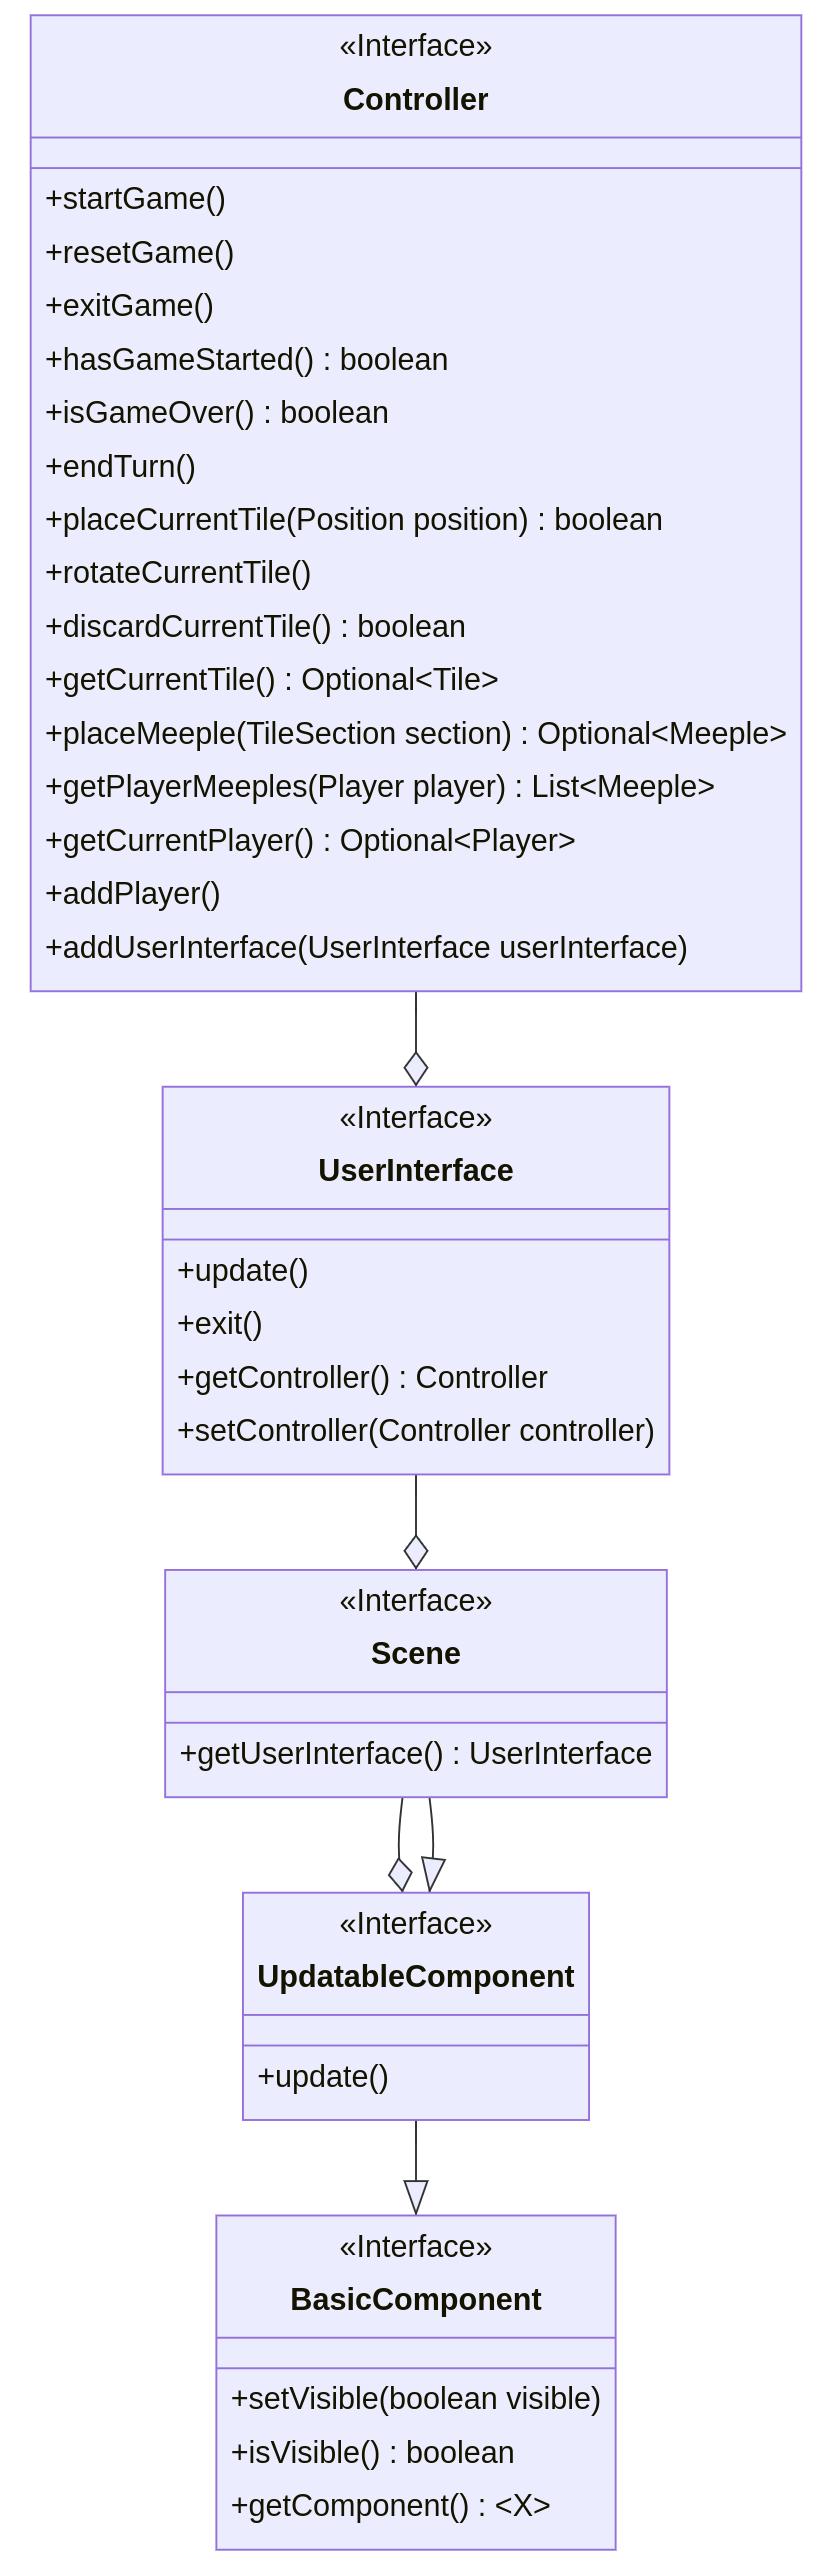
\includegraphics[scale=0.29]{images/design_uml.png}
    \caption{Schema UML architetturale.}
\end{figure}
\clearpage

\subsection{Design dettagliato}
\subsection*{Mauro Pellonara}

\subsubsection*{Permettere di sviluppare Meeple con diverse caratteristiche}
\begin{figure}[ht]
    \centering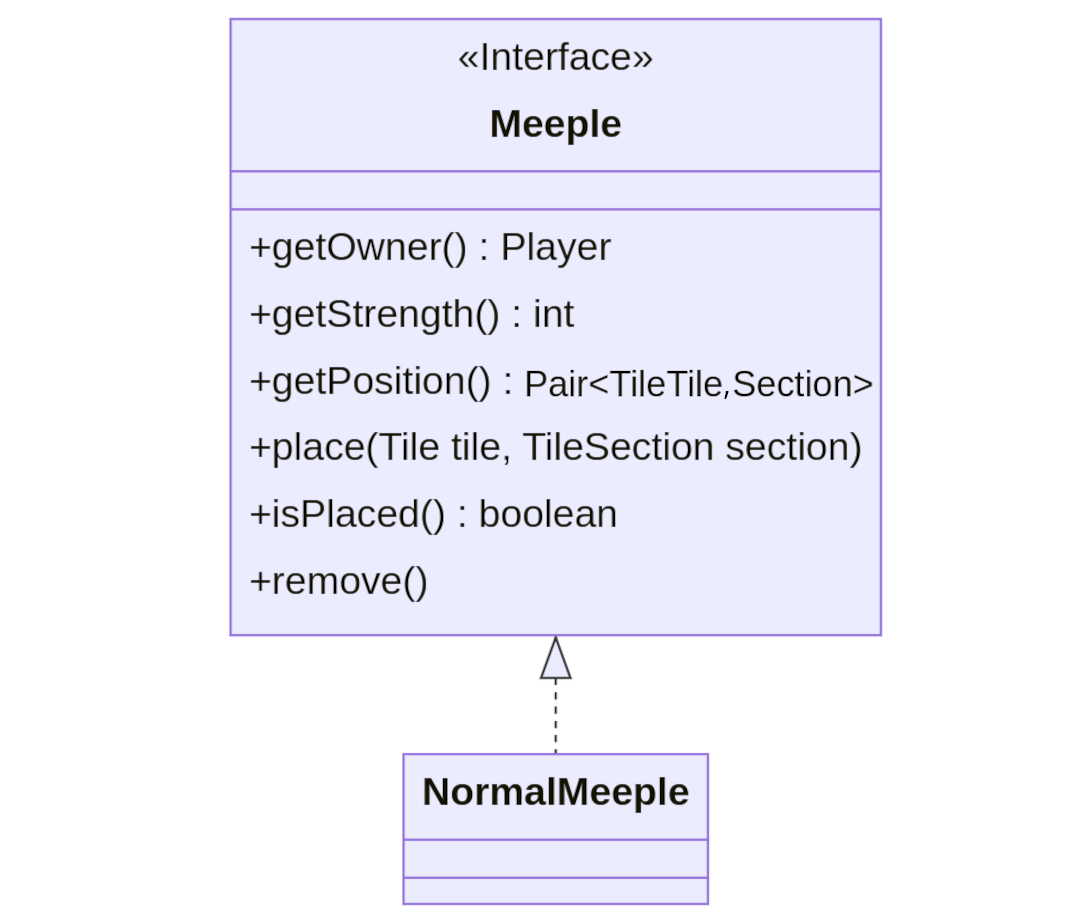
\includegraphics[scale=.25]{images/meeple.png}
    \caption{Rappresentazione UML dell'applicazione del pattern Strategy per Meeple e NormalMeeple.}
\end{figure}
\paragraph{Problema}
La versione classica del gioco supporta solo seguaci normali che non hanno funzioni speciali. Alcune espansioni introducono invece dei seguaci che valgono il doppio di quelli normali, è quindi necessario garantire espandibilità futura in caso di nuove espansioni.
\paragraph{Soluzione}
Usare il pattern Strategy sulla classe NormalMeeple introducendo un'interfaccia Meeple che può essere usata in futuro per introdurre nuovi seguaci di tipo diverso, un esempio sono quelli che hanno valore doppio rispetto ai normali.
\clearpage

\subsubsection*{Facilitare la creazione di istanze di MutableTile assieme ai relativi GameSet}
\begin{figure}[ht]
    \centering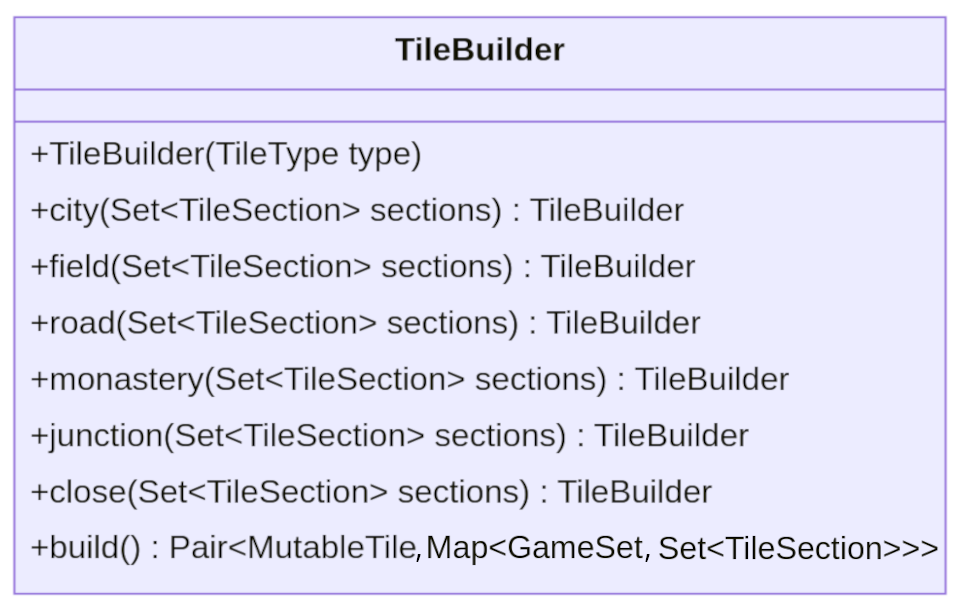
\includegraphics[scale=.30]{images/tilebuilder.png}
    \caption{Rappresentazione UML dell'applicazione del pattern Builder per MutableTile.}
\end{figure}
\paragraph{Problema}
Creare istanze di MutableTile assieme ai relativi GameSet in modo facile e leggibile.
\paragraph{Soluzione}
Usare il pattern Builder per la creazione di oggetti MutableTile rendendo più esplicite le istruzioni da eseguire. Assieme alla creazione di un'istanza di MutableTile possono anche essere creati i relativi GameSet e restituiti tutti assieme con il metodo build().
\clearpage

\subsubsection*{Facilitare la creazione di istanze di MutableTile di tipo diverso}
\begin{figure}[ht]
    \centering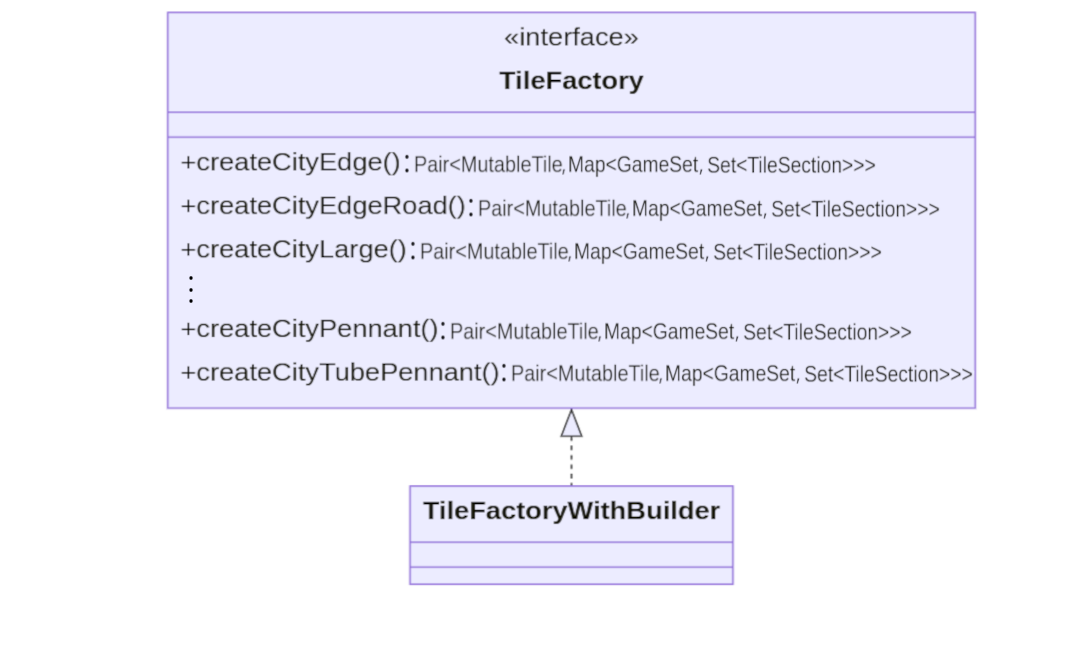
\includegraphics[scale=.35]{images/tilefactory.png}
    \caption{Rappresentazione UML dell'applicazione del pattern Factory Method per MutableTile.}
\end{figure}
\paragraph{Problema}
All'inizio di ogni partita vengono generate numerose MutableTile per ogni tipo, è quindi necessaria una procedura facile per la generazione di esse.
\paragraph{Soluzione}
TODO.
\clearpage

\subsubsection*{Evitare di tenere riferimenti doppi tra GameSet e Tile}
\begin{figure}[ht]
    \centering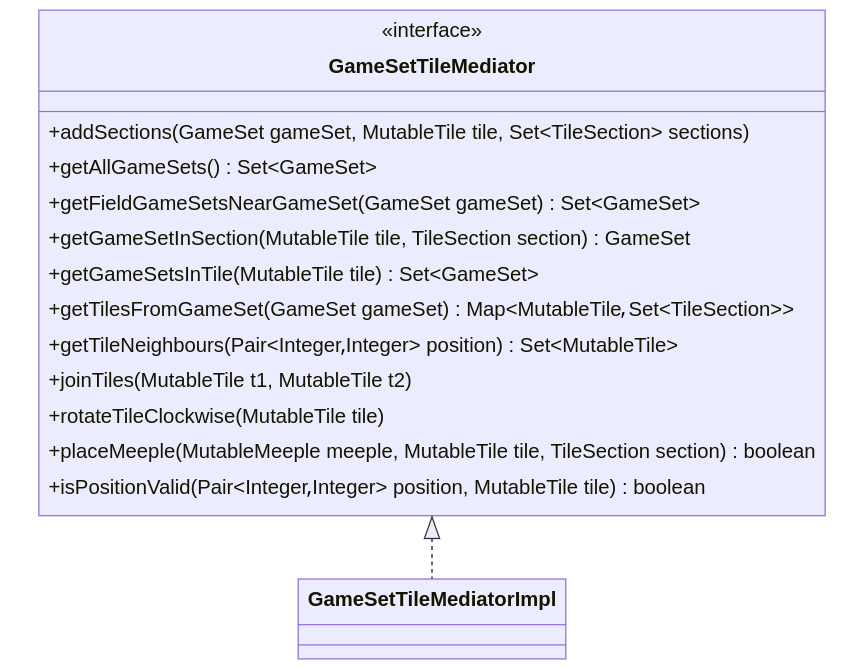
\includegraphics[scale=.35]{images/gamesettilemediator.png}
    \caption{Rappresentazione UML dell'applicazione del pattern Mediator per GameSet e Tile.}
\end{figure}
\paragraph{Problema}
TODO.
\paragraph{Soluzione}
TODO.
\clearpage

\subsubsection*{Permettere diversi tipi di campi di input per la creazione di Player}
\begin{figure}[ht]
    \centering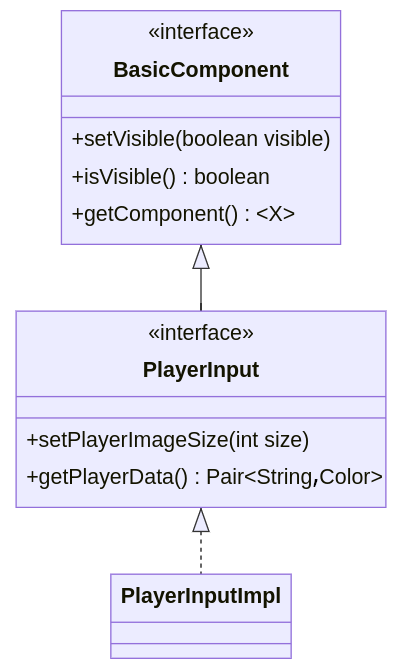
\includegraphics[scale=.35]{images/playerinput.png}
    \caption{Rappresentazione UML dell'applicazione del pattern Strategy per PlayerInput.}
\end{figure}
\paragraph{Problema}
Creare un componente grafico per l'inserimento delle informazioni necessarie alla creazione di un nuovo Player, rispettando quindi il Single Responsibility Principle. In oltre, far si che questo principio venga rispettato da qualsiasi view con interfaccia grafica.
\paragraph{Soluzione}
Creare una classe PlayerInputImpl che si occupa di ottenere e gestire le informazioni relative alla creazione di un nuovo Player. Ulteriormente, applicare il pattern Strategy alla classe PlayerInputImpl generalizzandone il comportamento e usando un tipo generico rappresentante il componente grafico utilizzato, che varia a seconda del GUI framework scelto.
\clearpage

\subsection*{Alessandro Martini}

\subsubsection*{Definizione di operazioni che vengono utilizzati su GameSet differenti}
\begin{figure}[ht]
    \centering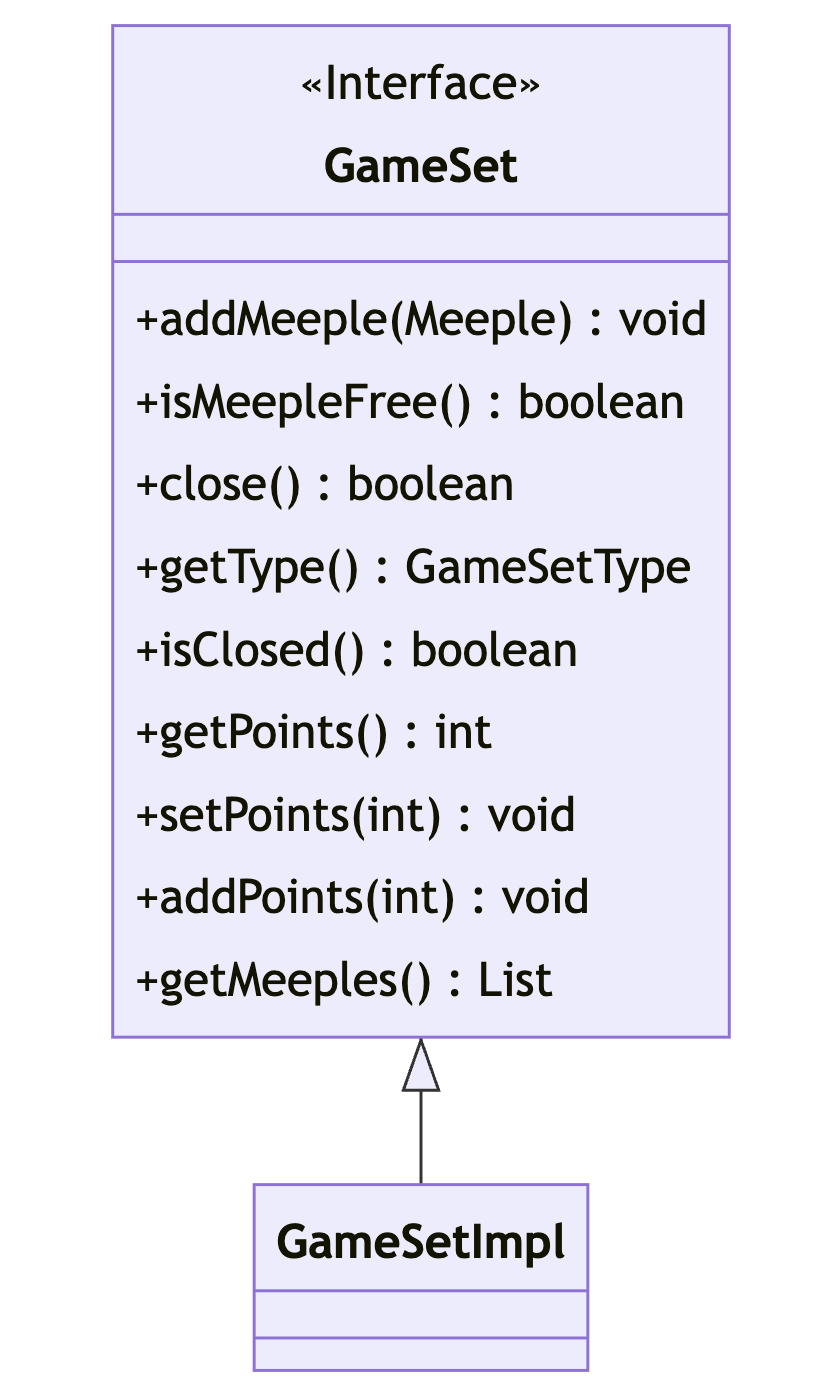
\includegraphics[scale=.4]{images/gameset.png}
    \caption{Rappresentazione UML dell'applicazione del pattern Strategy per GameSet e GameSetImpl}
\end{figure}
\paragraph{Problema:}
Assegnare logiche differenti per GameSet differenti. Si era posto il problema della scalabilità delle funzioni che ogni GameSet dovesse avere, anche per aggiornamenti futuri
\paragraph{Soluzione:}
Tramite il patter Strategy, sono andato a creare un'interfaccia GameSet che definisse le funzioni generali di ogni GameSet, così facendo, ho reso scalabile anche per upgrade futuri la possibilità di creare nuove funzioni e nuove regole per i vari tipi di GameSet.

\subsubsection*{Creazione di più GameSet con tipologie differenti}
\begin{figure}[ht]
    \centering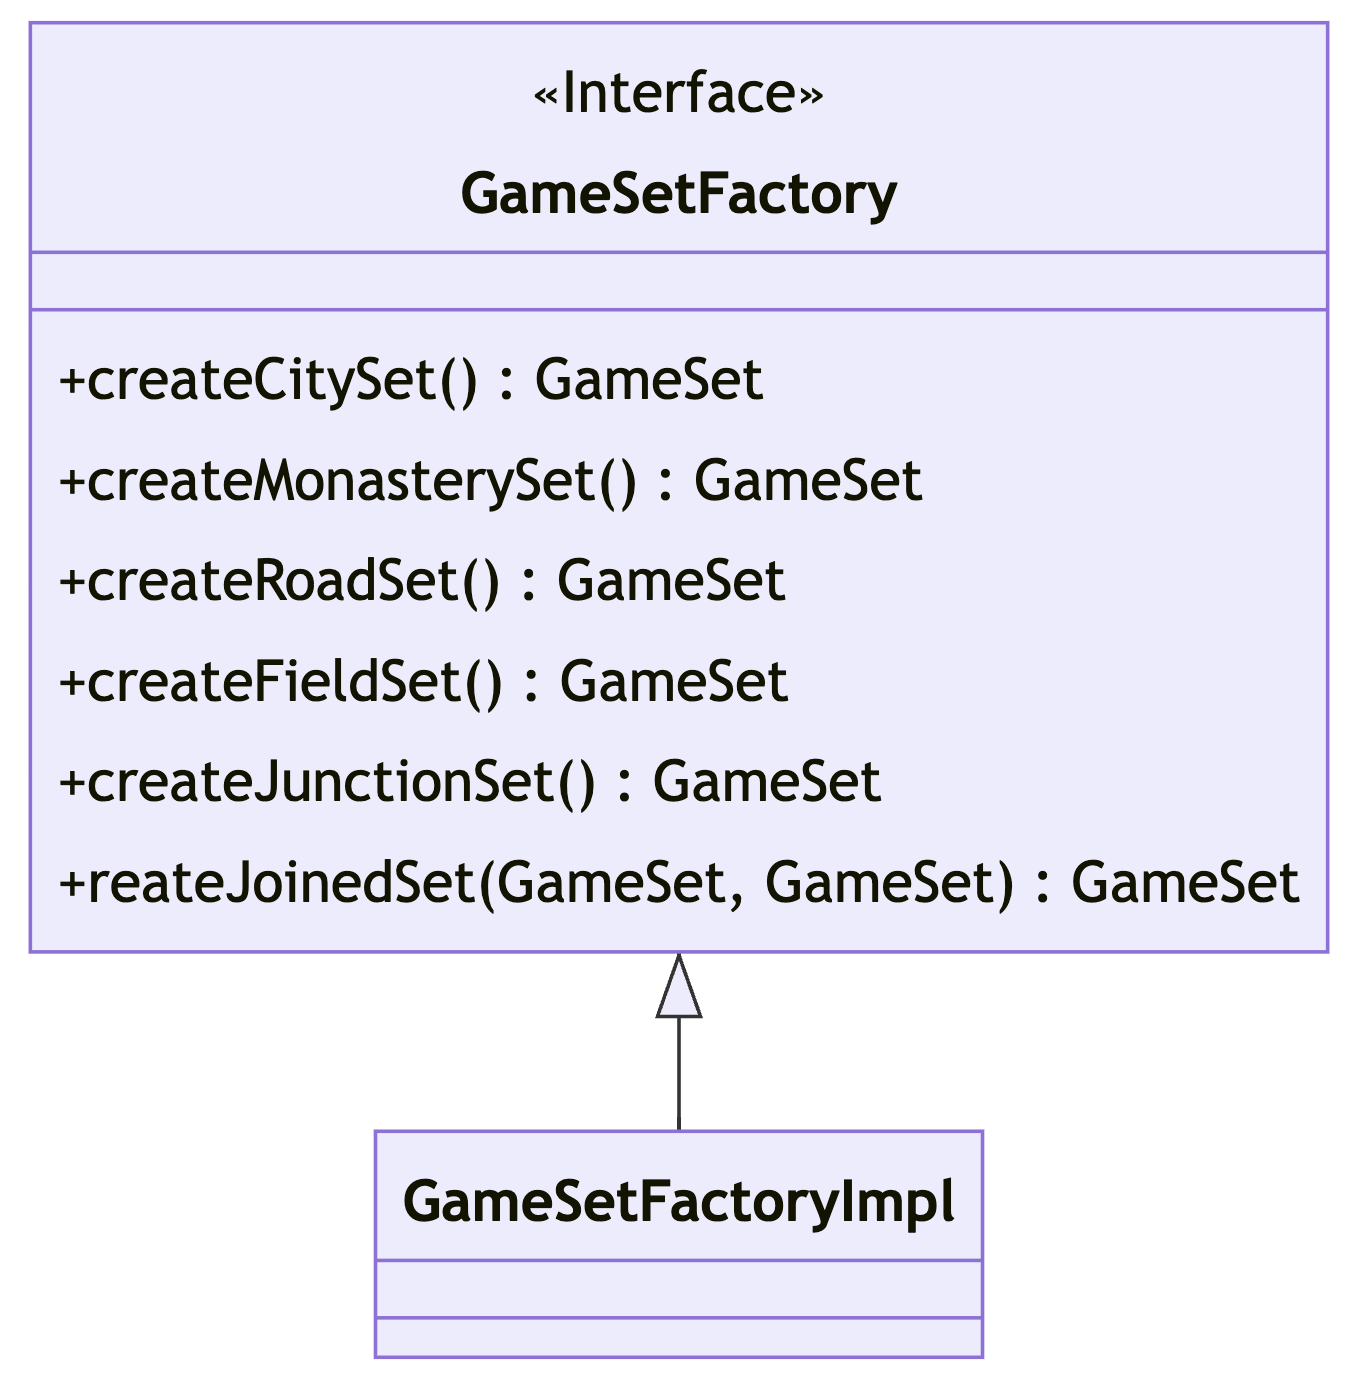
\includegraphics[scale=.3]{images/gamesetfactory.png}
    \caption{Rappresentazione UML dell'applicazione del pattern Strategy per il gamesetfactory e GameSetFactoryImpl}
\end{figure}

\paragraph{Problema:}
Creare una uguale implementazione di GameSet ma di tipi differenti
\paragraph{Soluzione:}
Tramite il pattern Strategy, siamo andati a implementare dei metodi che vanno a definire come i vari tipi di GameSet vengono creati, e inoltre come si possono creare dei GameSet da altri GameSet

\subsubsection*{Creazione di più BasicComponent con caratteristiche differenti}
\begin{figure}[ht]
    \centering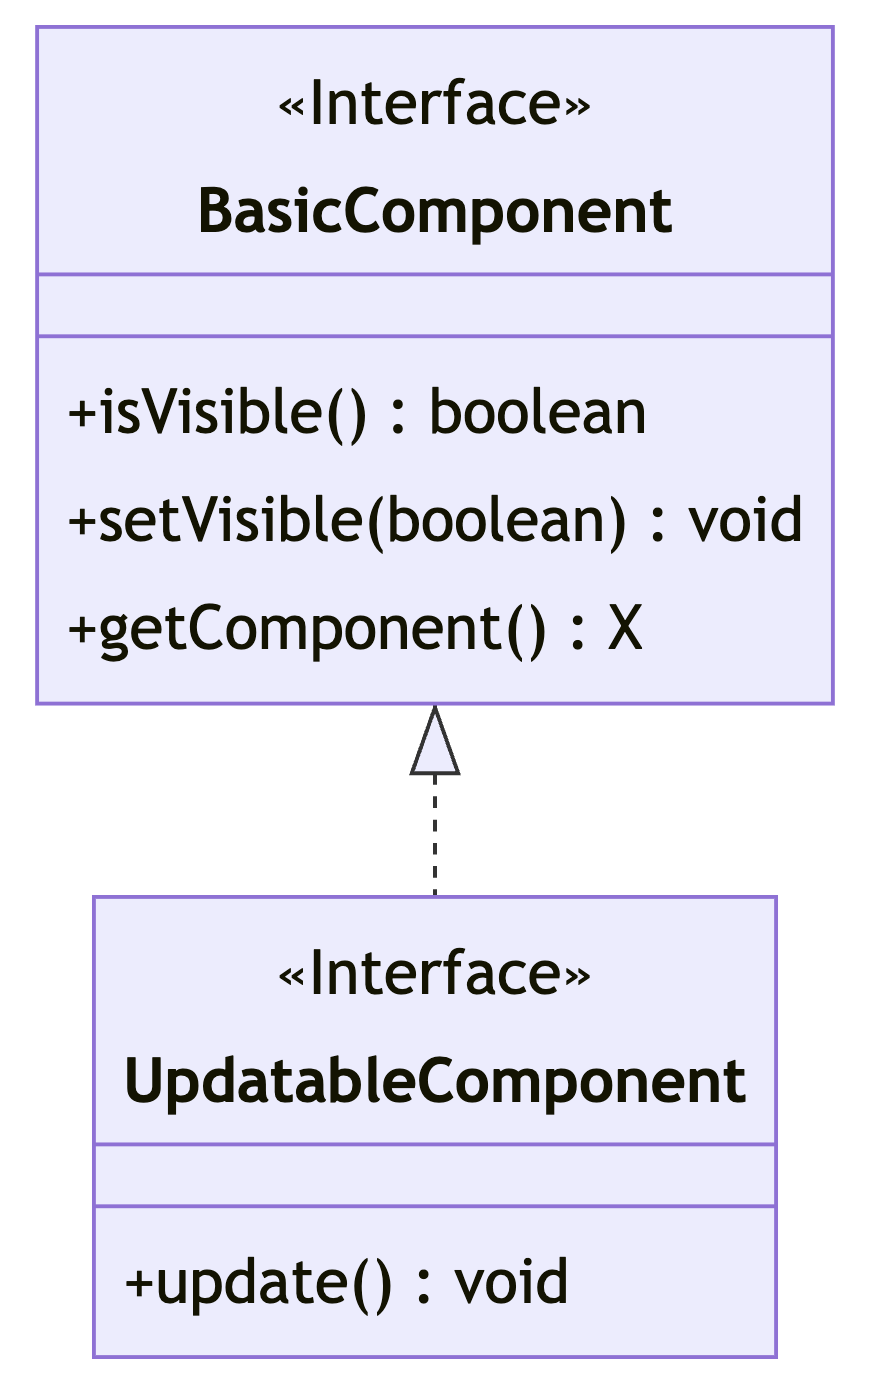
\includegraphics[scale=.5]{images/basiccomponent.png}
    \caption{Rappresentazione UML dell'applicazione del pattern Strategy per la classe interfaccia BasicComponent, che viene estesa da TileButton, a sua volta implementato da TileButtonImpl(Esempio)}
\end{figure}

\paragraph{Problema:}
La maggior parte dei componenti aveva dei metodi in comune, ma sviluppati in maniera differente a seconda dell'oggetto identificato nella view. (nell'esempio TileButton)
\paragraph{Soluzione:}
Sempre tramite il pattern Strategy, sono andato ad implementare i metodi che vanno a definire i comportamenti (metodi) in comune tra i vari componenti della view, e una estesa l'interfaccia, ogni metodo potrà sviluppare a suo piacimento i metodi presenti in BasicComponent.

\subsection*{Davide Speziali}

\subsection*{Samuele Giancarli}
\subsubsection*{Definizione di Tile}
\paragraph{Problema:}
\paragraph{Soluzione:}

\subsubsection*{Definizione di FooterComponent}
\paragraph{Problema:}
\paragraph{Soluzione:}

%
il posizionamento tessere è l'azione principale di tutto il gioco e la più complessa, in quanto bisognerà permettere il piazzamento solo nel caso in cui le tessere siano congiungibili.
%

Problema: piazzamento di una tessera



ecco cosa fa il getCurrentTile:

\begin{itemize}
\item va a verificare che la posizione selezionata non fosse stata già occupata da un’altra tessera, in caso negativo ritorna false
\item va a verificare che esista almeno una tile neighbour, in caso negativo ritorna false
\item va a verificare per ogni tile neighbour che la totalità delle section adiacenti alla current tile siano dello stesso tipo
\item solo dopo aver controllato ogni section di ogni neighbour e aver appurato che la current tile sia piazzabile allora: setPosition(position)
\item a questo punto ad ogni neighbour dovranno essere impostate a closed le section connesse con la current tile. La stessa cosa verrà fatta per le section della current tile connesse a quelle di un neighbour.
\subitem la struttura del ciclo è la stessa di quello precedente, ma è solo grazie al completamento del ciclo precedente che si avrà la sicurezza di poter impostare tutte le section a closed
\item (??????) solo a questo punto sarà possibile unire i gameset della tile corrente con quelli delle tile già presenti
\end{itemize}
